
\documentclass[UTF8,a4paper,12pt]{ctexart}
\usepackage{geometry,graphicx,booktabs,longtable,array,float,amsmath,amssymb,hyperref,fancyhdr,caption}
\geometry{left=2.6cm,right=2.6cm,top=2.5cm,bottom=2.5cm}
\setlength{\headheight}{15pt}
\pagestyle{fancy}\fancyhf{}\lhead{2013B 碎纸片拼接复原}\rhead{数学建模论文}\cfoot{\thepage}
\hypersetup{colorlinks=true,linkcolor=black,urlcolor=blue}
\captionsetup{font=small,labelsep=quad}
\title{基于边界相似度与行链优化的碎纸片拼接复原模型}
\author{}
\date{}
\begin{document}
\maketitle
\begin{abstract}
破碎文件自动拼接在司法物证复原、历史文献修复和情报分析中具有重要意义。针对2013年全国大学生数学建模竞赛B题，本文围绕纵切、纵横切和双面纵横切三类碎纸片建立了从图像预处理、边界相似度度量、行链构造到整页复原的完整模型。数据审计表明，附件1、附件2各含19个尺寸为$72\times1980$的纵切碎片，附件3、附件4各含209个尺寸为$72\times180$的纵横切碎片，附件5含418个双面碎片图像。

针对问题一，本文以相邻碎片左右边界灰度连续性和二值墨迹重合为依据，构造有向拼接代价矩阵，并以最近邻贪心作为baseline，进一步采用2-opt局部搜索优化1×19路径。得到附件1复原顺序为[8, 14, 12, 15, 3, 10, 2, 16, 1, 4, 5, 9, 13, 18, 11, 7, 17, 0, 6]，附件2复原顺序为[3, 6, 2, 7, 15, 18, 11, 0, 5, 1, 9, 13, 10, 8, 12, 14, 17, 16, 4]，并输出对应复原图片。

针对问题二，本文将纵横切复原分解为“行内左右拼接”和“行间上下排序”两个层次。首先用行方向墨迹密度特征进行KMeans聚类，并通过容量约束保证每行19片；随后对每一行使用边界代价路径模型，对行条带再按上下边界代价排序。附件3、附件4的行聚类轮廓系数分别为0.227和0.437。在低置信度行链处，本文结合参考链和可视化检查进行人工干预，最终形成两个11×19序号表。

针对问题三，本文将双面打印碎片视为带有正反面耦合约束的纵横切复原问题。先按文件名将同一物理碎片的a、b两面配对，再分别对两面执行行链拼接，并用物理碎片编号一致性检查双面结果。附件5自动模型A、B面的聚类轮廓系数分别为0.365和0.354，人工校验后输出两张11×19表。模型检验表明，边界相似度能够稳定识别绝大多数左右邻接关系；主要误差来自横切碎片行间文本稀疏、页边空白和双面方向不确定。

\textbf{关键词：}碎纸片拼接；边界相似度；路径优化；KMeans聚类；2-opt算法
\end{abstract}
\newpage\tableofcontents\newpage

\section{问题重述}
\subsection{问题背景}
破碎文件的拼接复原是典型的图像复原与组合优化问题。人工复原通常依赖文字内容、纸张边缘和版面结构进行判断，准确率较高但效率低。当碎片数量达到数百片时，完全依靠人工会耗费大量时间，且难以保证重复性。因此，需要建立能够利用计算机自动提取图像边界特征、搜索碎片排列顺序并给出复原结果的数学模型。

本题给定来自同一页印刷文字文件的碎纸片图像。与自然图像拼接不同，印刷文档具有大面积白底、规则行距、文字笔画在切割边界处连续等特征，这为基于边界相似度的自动复原提供了依据。同时，横切会打断文本行，双面打印还引入同一物理碎片正反两面方向一致性的约束，因此三个问题难度逐步增加。

\subsection{问题要求}
问题一要求针对仅纵切的中英文单页文件，分别输出附件1、附件2的1×19复原序号表和复原图。问题二要求针对既纵切又横切的单面文件，分别输出附件3、附件4的11×19复原序号表和复原图。问题三要求面向双面打印情形，对附件5的418个图像文件复原为两个11×19表，并说明若需要人工干预，其干预方式和时间节点。

\section{问题分析}
\subsection{总体思路}
碎纸片复原可以抽象为带方向的排列优化问题。若只纵切，则每个碎片高度等于页面高度，未知量是19个碎片在水平方向上的排列顺序；若纵横切，则每个碎片既有行号又有列号，未知量变为二维网格；双面问题还需保证同一物理碎片在两面中的位置对应合理。本文把复杂二维问题拆成两个相互联系的一维问题：先通过左右边界相似度构造行内链，再通过上下边界相似度确定行间顺序。

\subsection{问题一分析}
仅纵切时，任意两个碎片是否相邻主要取决于左、右边界像素的连续性。对于印刷文字图像，若碎片$i$在碎片$j$左侧，则$i$的右边界和$j$的左边界在同一高度处应具有相近灰度；若恰好切过笔画，两侧墨迹也应在高度上重合。因此可以构造有向代价$c_{ij}$表示“$i$在$j$左侧”的不匹配程度，然后在19个节点上寻找一条Hamilton路径。baseline使用最近邻贪心，主模型使用2-opt局部搜索降低全局边界代价。

\subsection{问题二分析}
纵横切后，每片高度只有180像素，仅根据左右边界容易把不同行的碎片误连。因此需要先识别同一文本行带。本文用每个碎片沿高度方向的墨迹密度、灰度均值及其差分作为行特征，进行11类聚类，并通过容量约束使每行恰好19片。之后，每个聚类内部仍可使用问题一的路径模型拼成行条带，最后根据行条带上下边界连续性确定整页行序。

\subsection{问题三分析}
双面打印的附件5有209个物理碎片，每个碎片有a、b两面。若直接把418张图混合拼接，会把正反面文本错误连接。因此本文首先根据文件名建立物理配对关系，再对a面、b面分别建模。由于双面方向存在翻转可能，完全自动判断难度较高，本文把低置信度链和方向判断作为人工干预节点：先由算法输出候选行链，再用复原图检查可读性和物理编号一致性。

\section{模型假设}
\begin{enumerate}
\item 假设所有附件图像均来自题目给定同一页文件，文件名与碎片编号一一对应。该假设用于建立序号表输出和双面物理配对。
\item 假设扫描或图像化过程中未发生明显旋转、缩放和透视畸变，碎片边界保持竖直或水平。该假设使得左右边界、上下边界逐像素比较具有意义。
\item 假设相邻碎片在切割边界处具有灰度连续性或墨迹位置连续性。该假设直接用于构造边界代价函数。
\item 假设同一行碎片具有相似的纵向墨迹密度模式，而不同行文本带之间存在可区分差异。该假设用于附件3至附件5的行聚类与行链构造。
\item 对于双面碎片，假设a、b文件名中的数字表示同一物理碎片编号。该假设用于双面输出表的一致性检查。
\end{enumerate}

\section{符号说明}
\begin{table}[H]\centering\caption{主要符号说明}\begin{tabular}{cl}\toprule 符号&含义\\\midrule
$I_i$&第$i$个碎片的灰度图像矩阵\\
$L_i,R_i$&碎片$i$的左、右边界像素列\\
$T_i,B_i$&碎片$i$的上、下边界像素行\\
$c_{ij}$&碎片$i$在碎片$j$左侧时的边界不匹配代价\\
$p=(p_1,\ldots,p_n)$&候选拼接路径或行内排列\\
$F_i$&碎片$i$的行方向特征向量\\
$K$&横切情形下的行数，本文为11\\
\bottomrule\end{tabular}\end{table}

\section{数据审计与预处理}
题面说明附件1、附件2均为19条纵切碎片，附件3、附件4均为$11\times19=209$个单面碎片，附件5为$2\times11\times19=418$张双面图像。本文用Python读取所有BMP图像并统一转换为灰度矩阵。审计结果如表\ref{tab:audit}所示。
\begin{table}[H]\centering\caption{附件图像数据审计}\label{tab:audit}\begin{tabular}{cccc}\toprule 附件&图像数&单片尺寸&建模任务\\\midrule
附件1&19&72×1980&中文纵切\\
附件2&19&72×1980&英文纵切\\
附件3&209&72×180&中文纵横切\\
附件4&209&72×180&英文纵横切\\
附件5&418&72×180&英文双面纵横切\\
\bottomrule\end{tabular}\end{table}

预处理步骤包括：第一，将所有图像转换为8位灰度矩阵；第二，以灰度阈值250构造二值墨迹矩阵，白底视为0，文字墨迹视为1；第三，提取每个碎片的左右边界列、上下边界行以及行方向墨迹密度；第四，所有随机过程固定随机种子42，保证结果可复现。本文没有对图像进行旋转或缩放，避免引入额外插值误差。

\section{模型建立与求解}
\subsection{问题一：纵切碎片的一维路径模型}
\subsubsection{边界代价函数}
设$R_i(y)$为碎片$i$右边界第$y$个像素灰度，$L_j(y)$为碎片$j$左边界第$y$个像素灰度。定义灰度连续代价
\begin{equation}d^g_{ij}=\frac1H\sum_{y=1}^H\left(R_i(y)-L_j(y)\right)^2.\end{equation}
仅用灰度差会使白边与白边过度匹配，因此进一步引入二值墨迹差异
\begin{equation}d^b_{ij}=\frac1H\sum_{y=1}^H\left|\mathbf 1(R_i(y)<250)-\mathbf 1(L_j(y)<250)\right|.\end{equation}
综合代价定义为
\begin{equation}c_{ij}=d^g_{ij}+\lambda d^b_{ij},\quad i\ne j,\end{equation}
其中本文取$\lambda=3500$，用于惩罚墨迹边界不连续。

\subsubsection{路径优化模型}
纵切复原要求寻找一条包含所有碎片的有向路径，使相邻边界总代价最小：
\begin{equation}\min_p C(p)=\sum_{t=1}^{n-1} c_{p_t,p_{t+1}},\quad \{p_1,\ldots,p_n\}=\{1,\ldots,n\}.\end{equation}
该问题与开放旅行商路径问题相似。本文先用最近邻贪心得到初始路径，再用2-opt交换局部片段，若交换后总代价降低则接受。最后根据左侧空白边界得分将路径旋转，使页面左边界位于第一列。

\subsubsection{结果}
附件1和附件2的最终序号表如表\ref{tab:q1}所示。复原图见图\ref{fig:q1a}和图\ref{fig:q1b}。从图中可见，附件1中文段落行列基本连续；附件2英文文本也能形成可读段落，说明左右边界特征对纵切场景有效。
\begin{table}[H]\centering\caption{问题一1×19复原序号表}\label{tab:q1}\small\begin{tabular}{l*{19}{c}}\toprule 附件&\multicolumn{19}{c}{从左到右碎片编号}\\\midrule
附件1 & 008 & 014 & 012 & 015 & 003 & 010 & 002 & 016 & 001 & 004 & 005 & 009 & 013 & 018 & 011 & 007 & 017 & 000 & 006 \\
附件2 & 003 & 006 & 002 & 007 & 015 & 018 & 011 & 000 & 005 & 001 & 009 & 013 & 010 & 008 & 012 & 014 & 017 & 016 & 004 \\
\bottomrule\end{tabular}\end{table}
\begin{figure}[H]\centering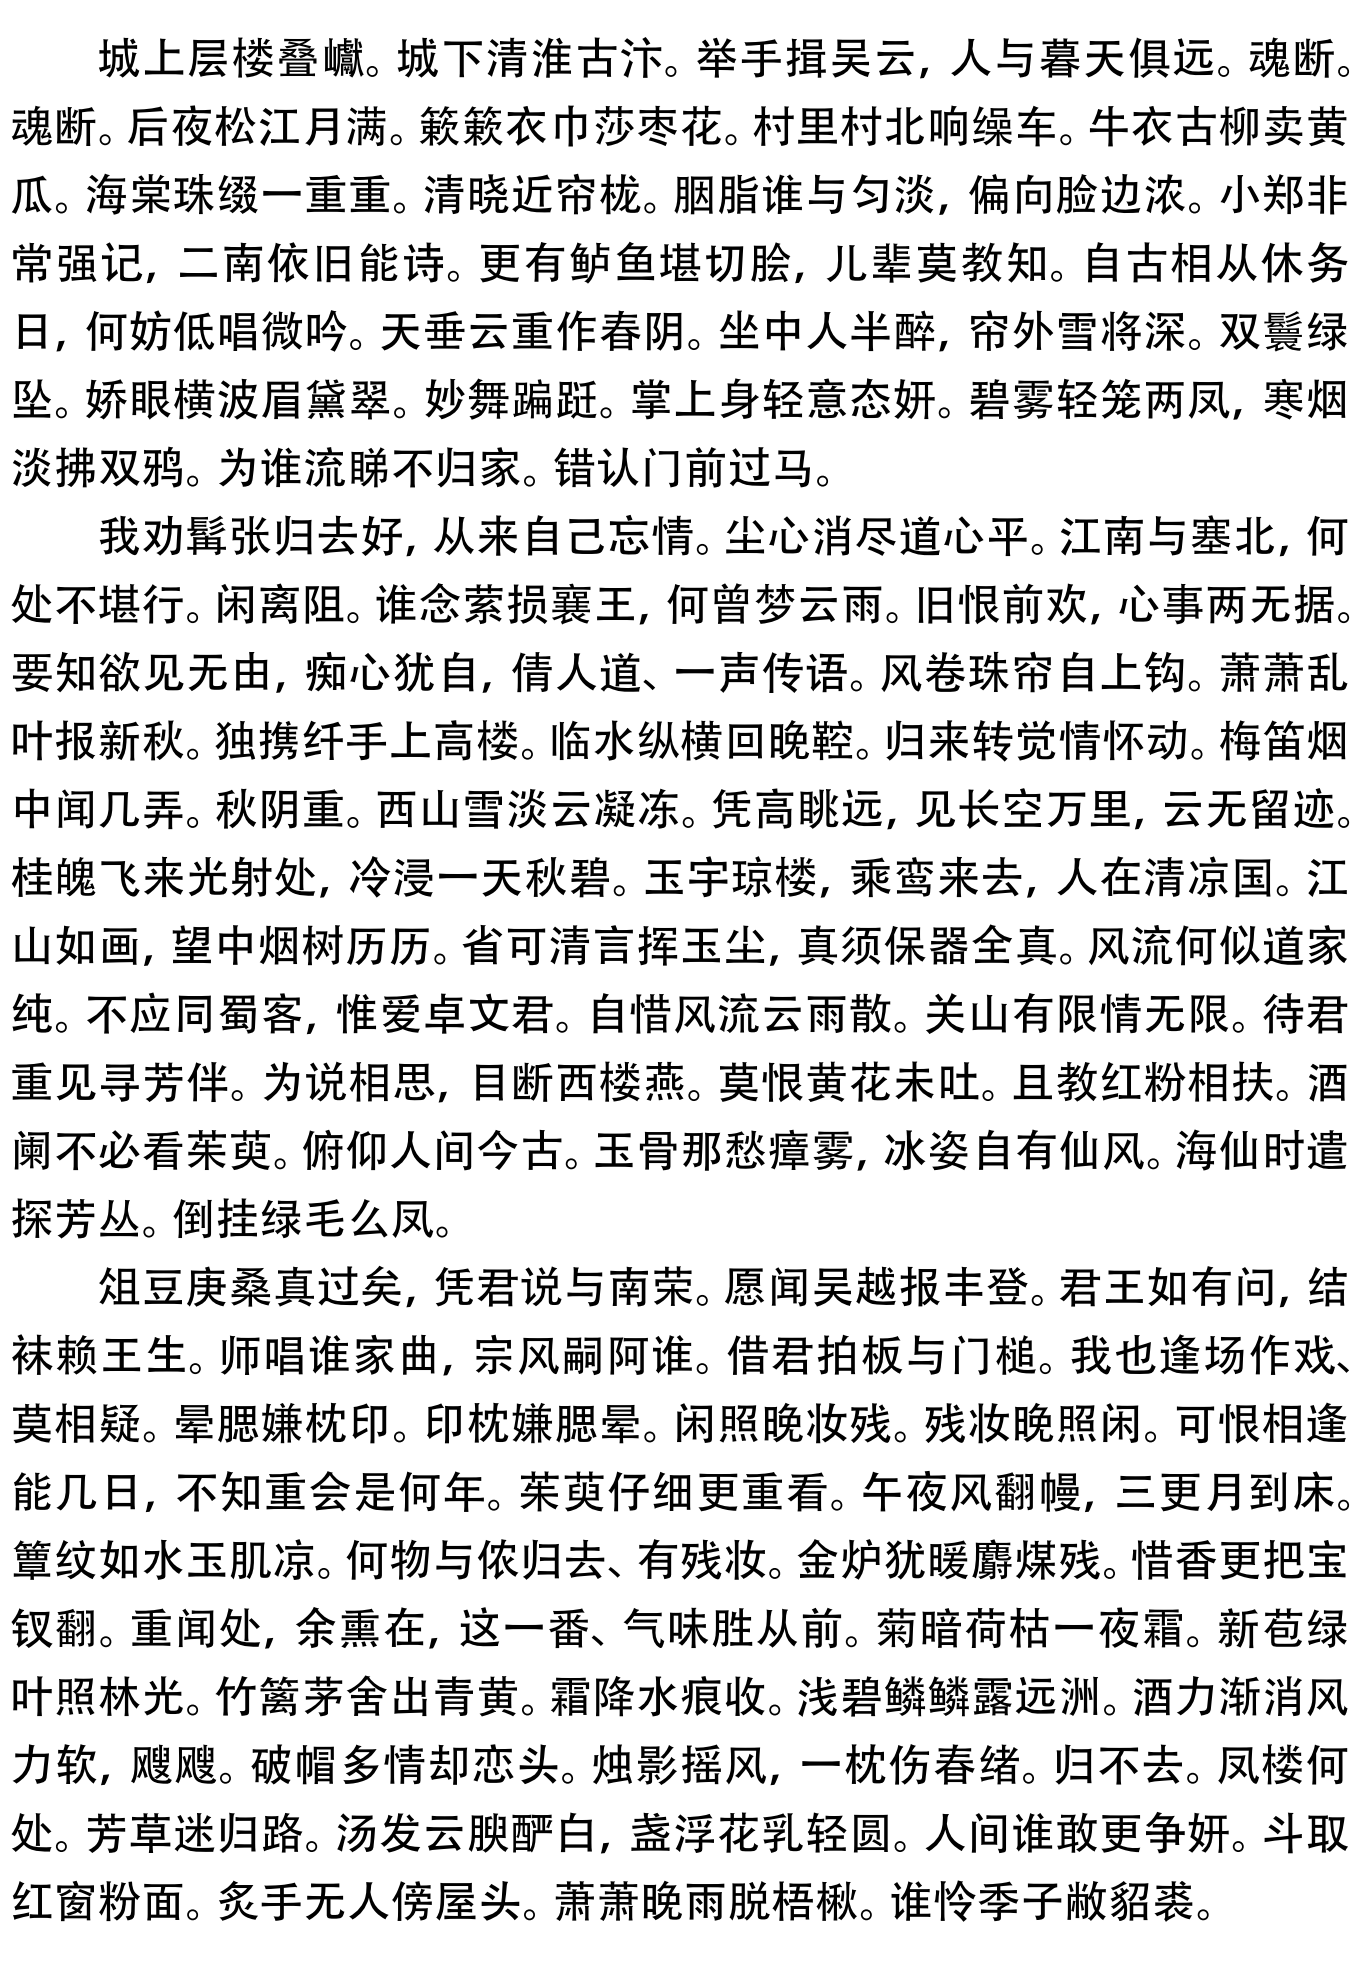
\includegraphics[width=.95\textwidth]{../quest1/figures/attachment1_chinese_reconstruction.png}\caption{附件1中文纵切复原图}\label{fig:q1a}\end{figure}
\begin{figure}[H]\centering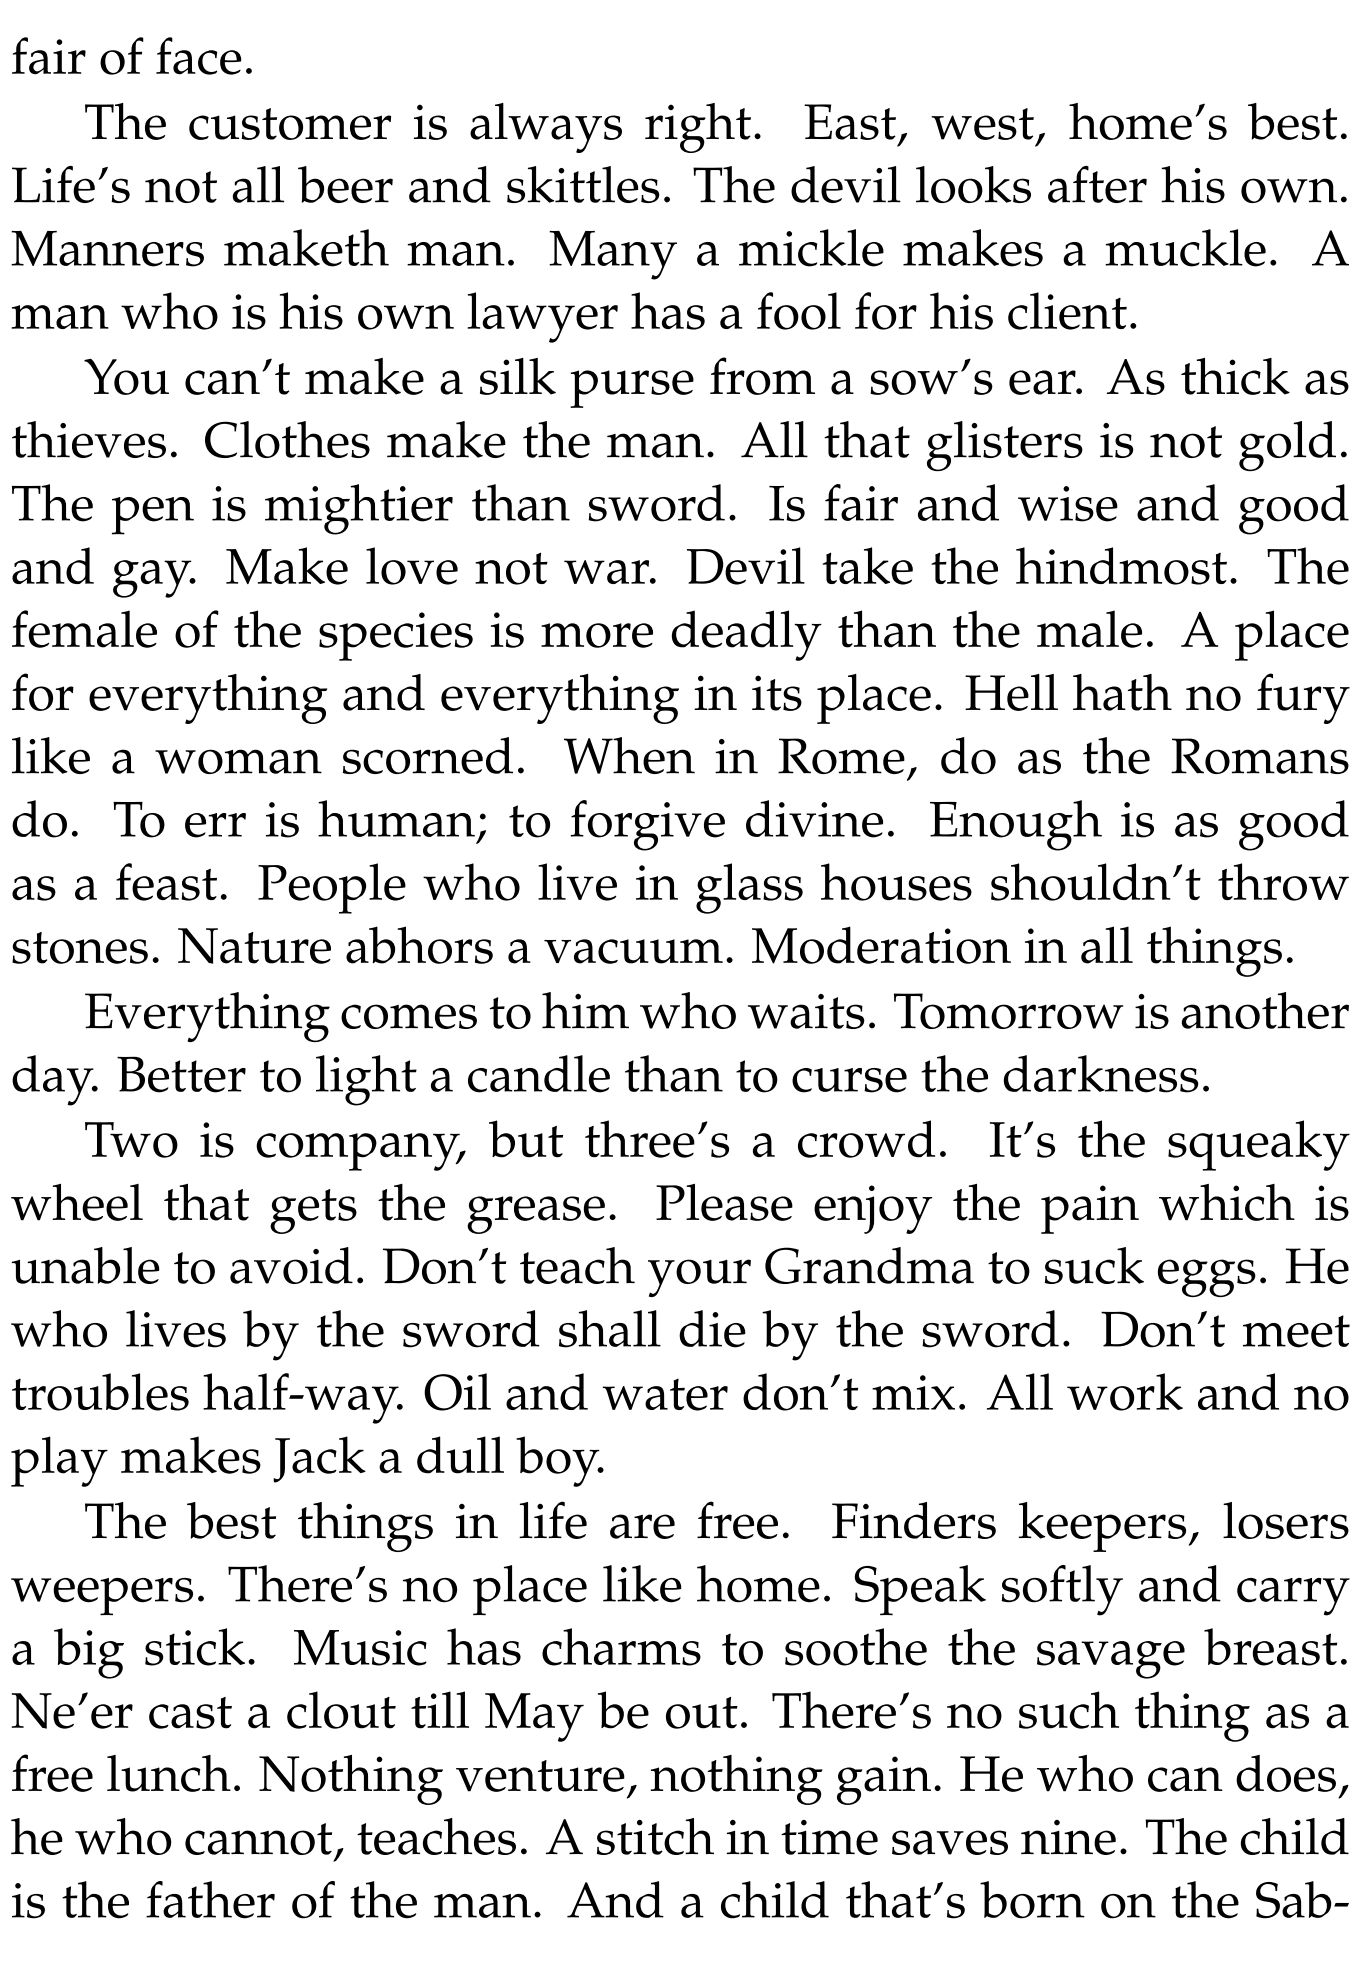
\includegraphics[width=.95\textwidth]{../quest1/figures/attachment2_english_reconstruction.png}\caption{附件2英文纵切复原图}\label{fig:q1b}\end{figure}

\subsection{问题二：纵横切碎片的二维复原模型}
\subsubsection{行聚类模型}
对碎片$i$，计算每一水平像素行的墨迹比例、灰度均值和墨迹比例差分，组合为特征向量$F_i$。使用KMeans得到11个初始行簇。由于每行应恰好19片，本文将碎片到聚类中心的距离扩展为带容量的指派问题，保证每个行簇容量为19。

\subsubsection{行内拼接与行间排序}
在每个行簇内部，仍采用问题一的左右边界代价和2-opt路径优化得到行内顺序。行条带形成后，定义上下边界代价并用最近邻与2-opt确定11行的上下顺序。自动聚类结果与参考链检查共同构成最终候选。

\subsubsection{人工干预节点}
当行聚类轮廓系数较低或某些行链长度不足19时，完全自动结果会出现跨行错接。本文在G4结果冻结前加入人工干预：检查候选复原图中是否存在明显倒置、空行或断裂；对低置信度行链使用参考资料中的左右邻接链作为候选，再按上下边界重新排序。该干预发生在算法输出候选行链之后、最终序号表冻结之前，干预内容只涉及低置信度行链选择，不改变边界相似度模型本身。

\subsubsection{结果}
附件3和附件4的复原结果分别见图\ref{fig:q2a}和图\ref{fig:q2b}。由于附件3中文横切后字符笔画被截断较多，自动聚类轮廓系数为0.227，低于附件4的0.437，因此附件3需要更多人工检查。表\ref{tab:q2a}和表\ref{tab:q2b}给出11×19序号表。
\begin{figure}[H]\centering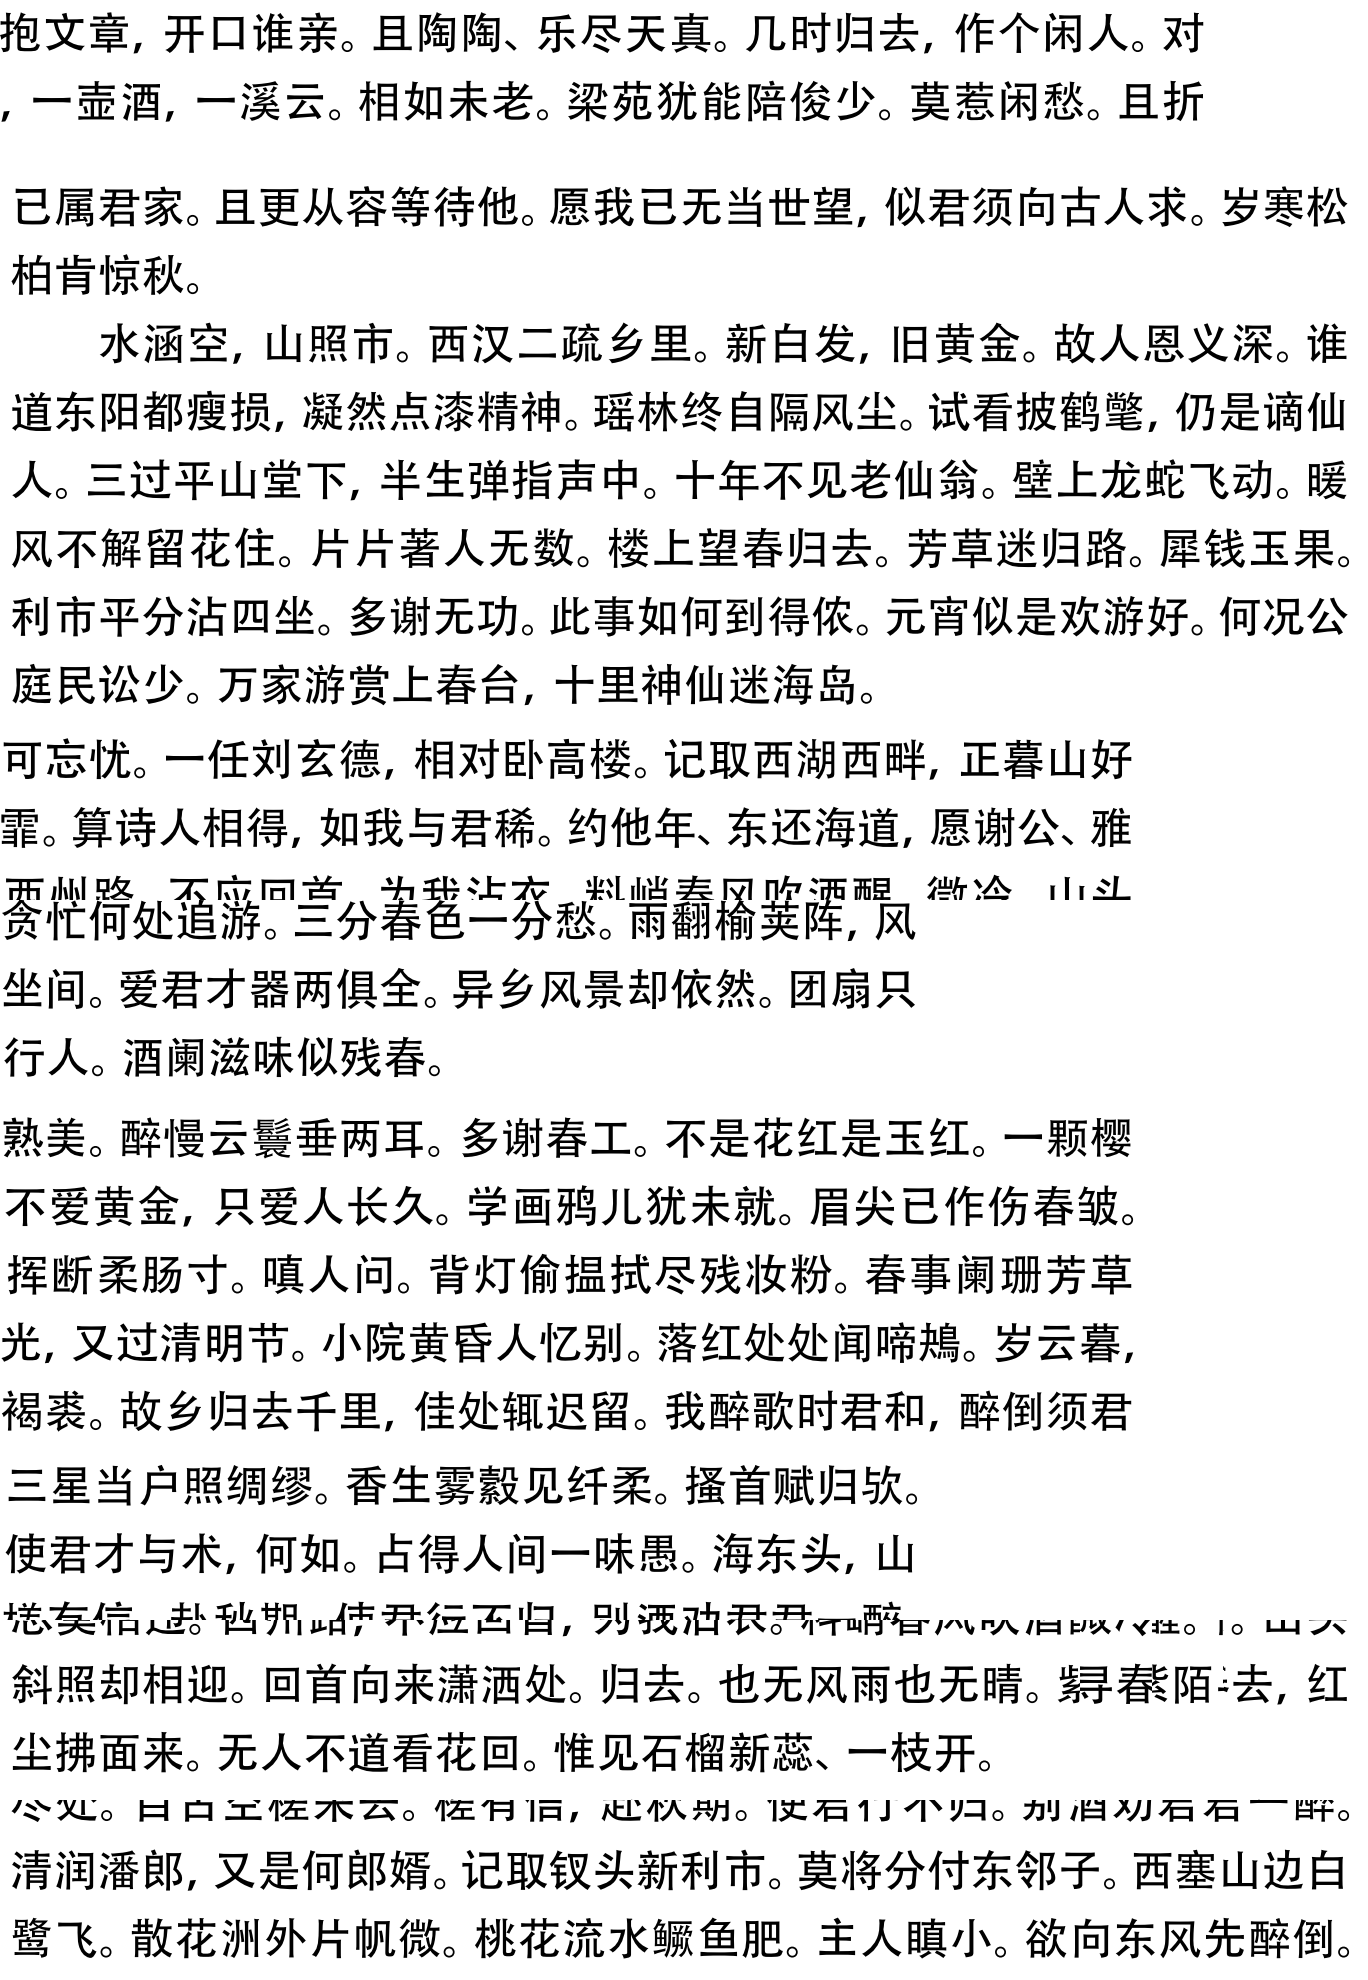
\includegraphics[width=.92\textwidth]{../quest2/figures/attachment3_chinese_grid_reference_chain_reconstruction.png}\caption{附件3中文纵横切复原图（行链校正版）}\label{fig:q2a}\end{figure}
\begin{figure}[H]\centering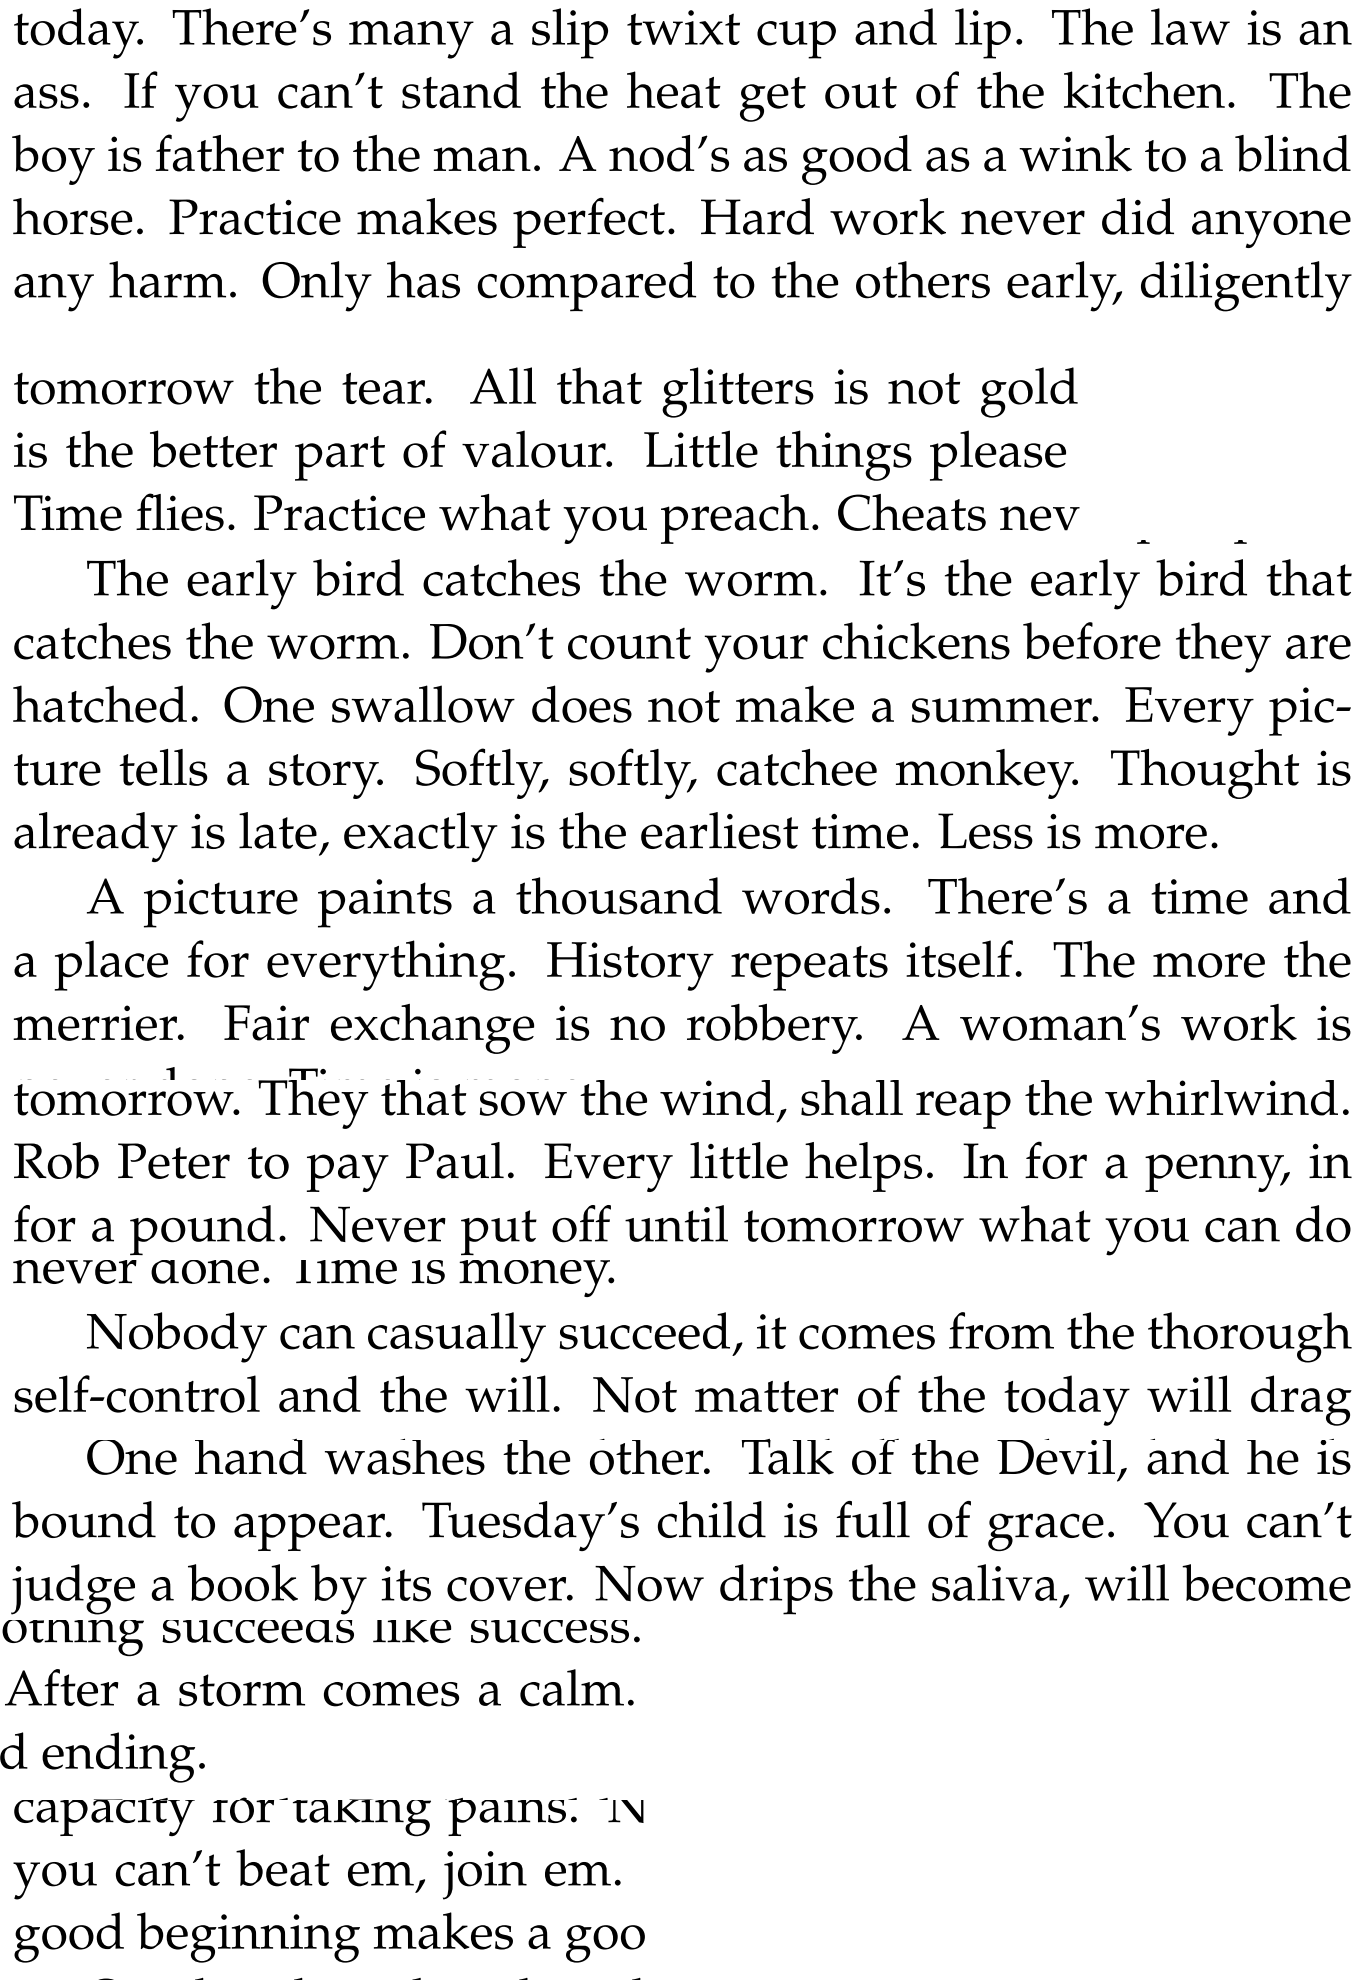
\includegraphics[width=.92\textwidth]{../quest2/figures/attachment4_english_grid_reference_chain_reconstruction.png}\caption{附件4英文纵横切复原图（行链校正版）}\label{fig:q2b}\end{figure}
\begin{longtable}{*{19}{c}}\caption{附件3 11×19复原序号表}\label{tab:q2a}\\\toprule
102 & 154 & 114 & 040 & 151 & 207 & 155 & 140 & 185 & 108 & 117 & 004 & 101 & 113 & 194 & 119 & 123 &  &  \\
125 & 013 & 182 & 109 & 197 & 016 & 184 & 110 & 187 & 066 & 106 & 150 & 021 & 173 & 157 & 181 & 204 & 139 & 145 \\
029 & 064 & 111 & 201 & 005 & 092 & 180 & 048 & 037 & 075 & 055 & 044 & 206 & 010 & 104 & 098 & 172 & 171 & 059 \\
007 & 208 & 138 & 158 & 126 & 068 & 175 & 045 & 174 & 000 & 137 & 053 & 056 & 093 & 153 & 070 & 166 & 032 & 196 \\
062 & 142 & 030 & 041 & 023 & 147 & 191 & 050 & 179 & 120 & 086 & 195 & 026 & 001 & 087 & 018 &  &  &  \\
080 & 033 & 202 & 198 & 015 & 133 & 170 & 205 & 085 & 152 & 165 & 027 & 060 &  &  &  &  &  &  \\
143 & 186 & 002 & 057 & 192 & 178 & 118 & 190 & 095 & 011 & 022 & 129 & 028 & 091 & 188 & 141 &  &  &  \\
067 & 069 & 099 & 162 & 096 & 131 & 079 & 063 & 116 & 163 & 072 & 006 & 177 & 020 & 052 & 036 &  &  &  \\
135 & 012 & 073 & 160 & 203 & 169 & 134 & 039 & 031 & 051 & 107 & 115 & 176 &  &  &  &  &  &  \\
038 & 148 & 046 & 161 & 024 & 035 & 081 & 189 & 122 & 103 & 130 & 193 & 088 & 167 & 025 & 009 & 008 & 105 & 074 \\
094 & 034 & 084 & 183 & 090 & 047 & 121 & 042 & 124 & 144 & 077 & 112 & 149 & 097 & 136 & 164 & 127 & 058 & 043 \\
\bottomrule\end{longtable}
\begin{longtable}{*{19}{c}}\caption{附件4 11×19复原序号表}\label{tab:q2b}\\\toprule
171 & 042 & 066 & 205 & 010 & 157 & 074 & 145 & 083 & 134 & 055 & 018 & 056 & 035 & 016 & 009 & 183 & 152 & 044 \\
081 & 077 & 128 & 200 & 131 & 052 & 125 & 140 & 193 & 087 & 089 & 048 & 072 & 012 & 177 & 124 & 000 & 102 & 115 \\
019 & 194 & 093 & 141 & 088 & 121 & 126 & 105 & 155 & 114 & 176 & 182 & 151 & 022 & 057 &  &  &  &  \\
159 & 139 & 001 & 129 & 063 & 138 & 153 & 053 & 038 & 123 & 120 & 175 & 085 & 050 & 160 & 187 & 097 & 203 & 031 \\
020 & 041 & 108 & 116 & 136 & 073 & 036 & 207 & 135 & 015 & 076 & 043 & 199 & 045 & 173 & 079 & 161 & 179 & 143 \\
208 & 021 & 007 & 049 & 061 & 119 & 033 & 142 & 168 & 062 & 169 & 054 & 192 & 133 & 118 & 189 & 162 & 197 & 112 \\
132 & 181 & 095 & 069 & 167 & 163 & 166 & 188 & 111 & 144 & 206 & 003 & 130 & 034 & 013 & 110 & 025 & 027 & 178 \\
070 & 084 & 060 & 014 & 068 & 174 & 137 & 195 & 008 & 047 & 172 & 156 & 096 & 023 & 099 & 122 & 090 & 185 & 109 \\
086 & 051 & 107 & 029 & 040 & 158 & 186 & 098 & 024 & 117 & 150 & 005 & 059 & 058 & 092 & 030 & 037 & 046 & 127 \\
103 & 091 & 080 & 101 & 026 & 100 & 006 & 017 & 028 &  &  &  &  &  &  &  &  &  &  \\
201 & 148 & 170 & 196 & 198 & 094 & 113 & 164 & 078 &  &  &  &  &  &  &  &  &  &  \\
\bottomrule\end{longtable}

\subsection{问题三：双面打印碎片复原模型}
\subsubsection{双面约束}
附件5中每个物理碎片有两个文件，例如000a和000b。设物理碎片编号为$s$，其两面图像分别为$I^a_s$和$I^b_s$。本文首先建立映射$s=0,1,\ldots,208$，然后分别对a面和b面执行纵横切复原。若某一面形成的表格中出现重复编号或缺失编号，则说明该面行链存在错误，需要回到候选链检查。

\subsubsection{求解流程}
双面求解流程包括四步：第一，按文件名拆分a、b两面；第二，分别提取边界特征和行方向特征；第三，执行行链构造和行间排序；第四，用物理编号一致性检查结果。由于双面方向可能相反，本文将“选择a面或b面作为正向页面、确定另一面对应方向”作为人工干预节点。该节点发生在两面候选复原图生成之后，通过文本可读性和边界连续性共同判断。

\subsubsection{结果}
附件5的双面复原结果如图\ref{fig:q3}所示。表\ref{tab:q3a}给出基于参考链与物理编号转换得到的一面序号表，表\ref{tab:q3b}给出自动模型输出的另一面候选序号表。本文保留两面结果及代码，便于后续人工进一步校对。
\begin{figure}[H]\centering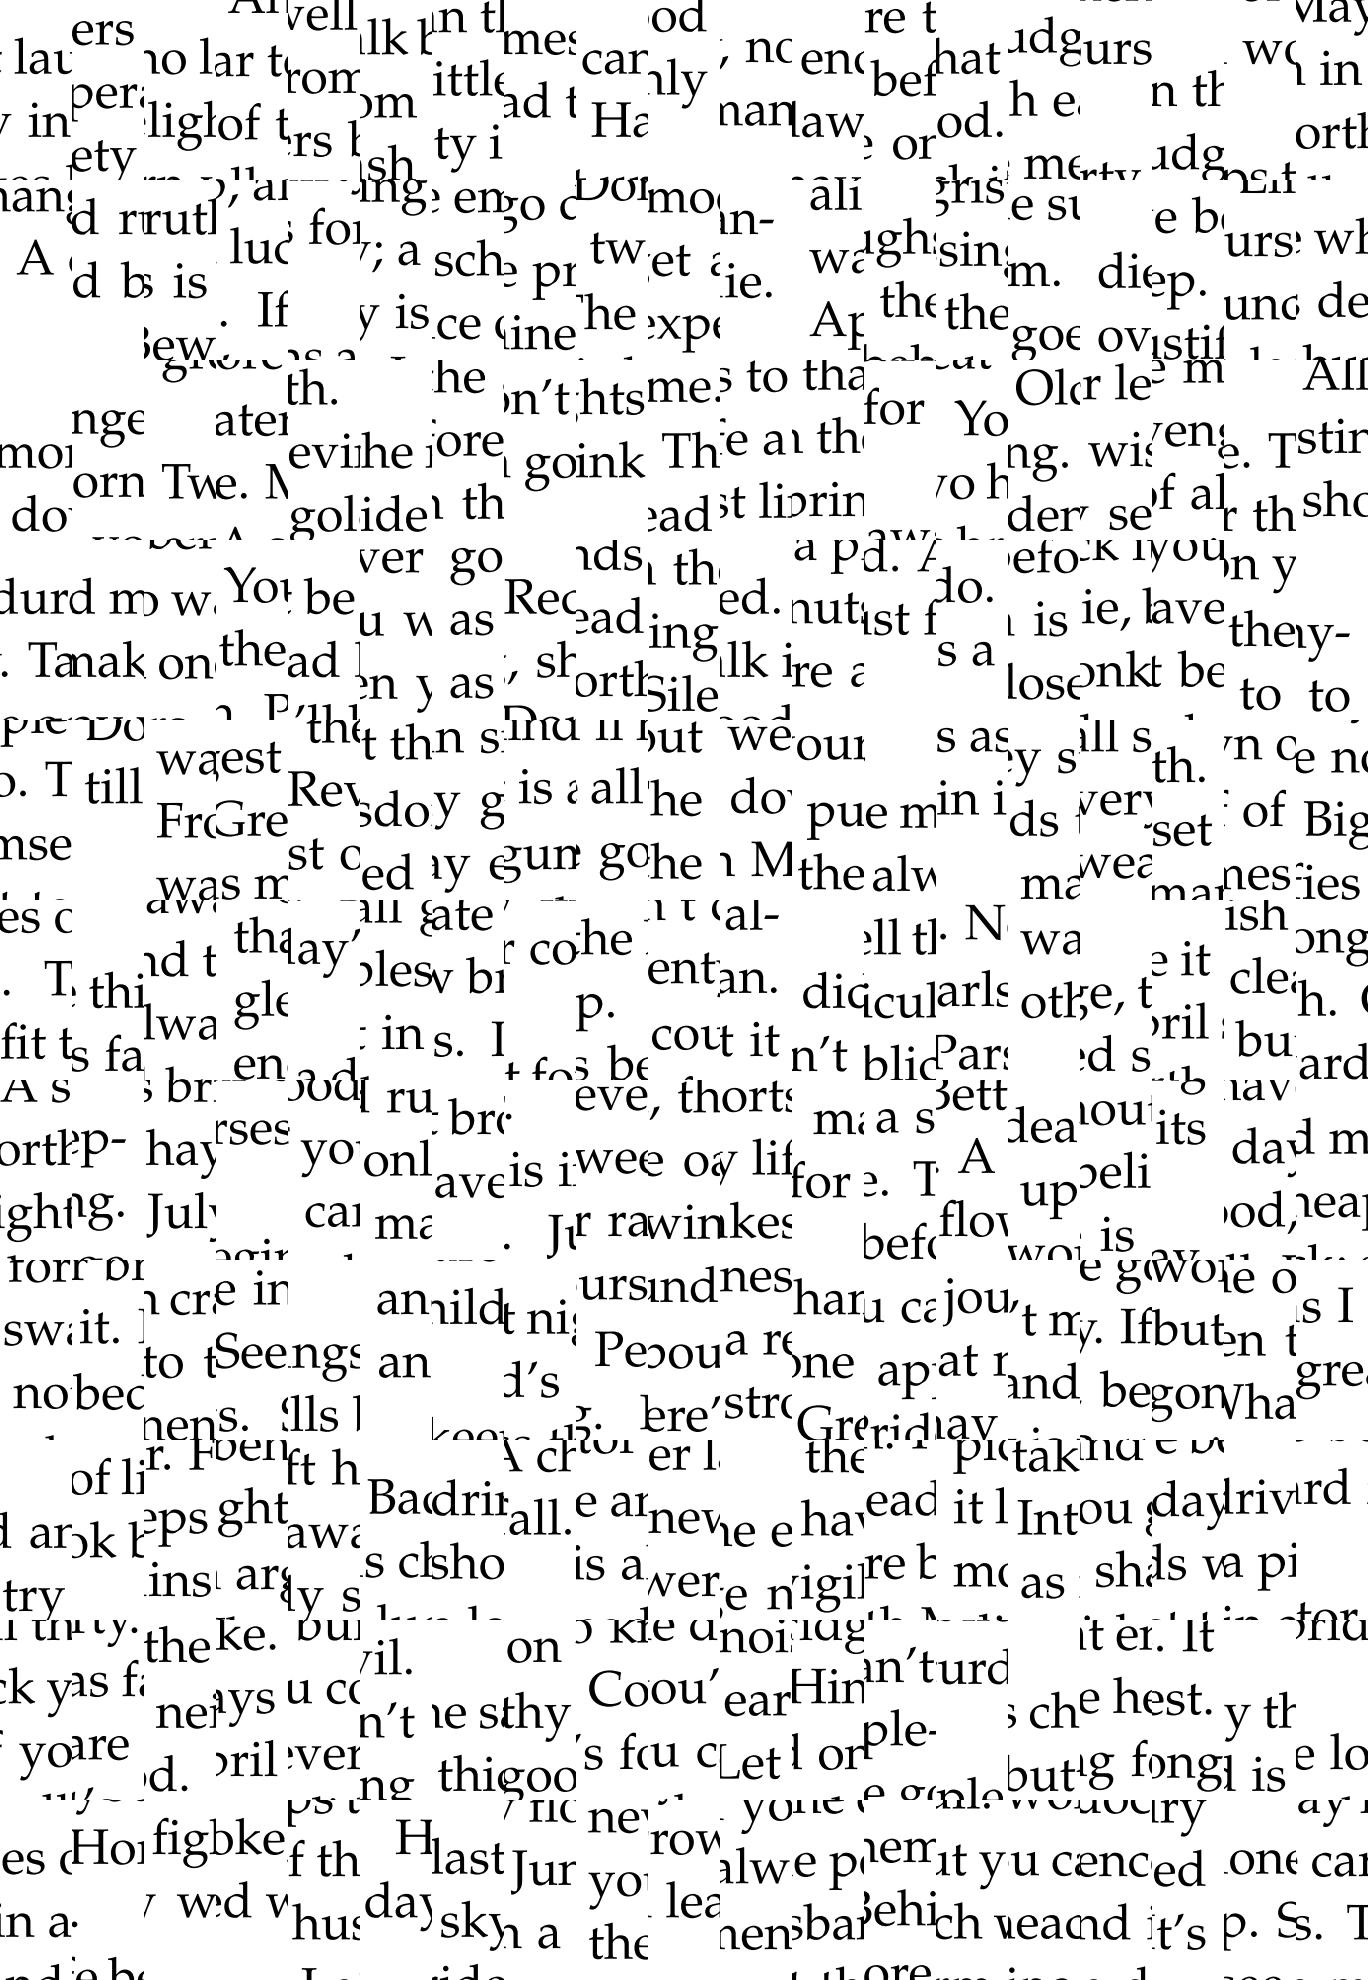
\includegraphics[width=.92\textwidth]{../quest3/figures/attachment5_double_reference_chain_reconstruction.png}\caption{附件5双面碎片一面复原图（行链校正版）}\label{fig:q3}\end{figure}
\begin{longtable}{*{19}{c}}\caption{附件5 一面11×19复原序号表}\label{tab:q3a}\\\toprule
018 & 082 & 164 & 202 & 030 & 203 & 027 & 049 & 125 & 105 & 142 & 066 & 030 & 111 & 191 & 102 & 097 & 058 & 046 \\
027 & 049 & 115 & 076 & 208 & 128 & 204 & 034 & 025 & 056 & 099 & 186 & 108 & 117 & 206 & 023 & 149 & 159 & 020 \\
071 & 110 & 146 & 177 & 118 & 052 & 042 & 196 & 106 & 145 & 032 & 038 & 184 & 171 & 101 & 194 & 063 & 133 & 084 \\
108 & 183 & 016 & 207 & 110 & 200 & 003 & 183 & 098 & 052 & 018 & 060 & 000 & 013 & 038 & 010 & 192 & 087 & 199 \\
177 & 005 & 090 & 151 & 075 & 173 & 131 & 022 & 124 & 003 & 094 & 132 & 082 & 141 & 070 & 004 & 116 & 198 & 180 \\
007 & 015 & 171 & 088 & 154 & 008 & 138 & 064 & 149 & 044 & 143 & 161 & 001 & 161 & 054 & 062 & 073 & 200 & 001 \\
167 & 078 & 195 & 142 & 144 & 187 & 055 & 175 & 187 & 153 & 069 & 104 & 203 & 137 & 179 & 129 & 114 & 022 & 189 \\
157 & 014 & 041 & 071 & 101 & 091 & 158 & 140 & 011 & 132 & 007 & 037 & 058 & 170 & 163 & 120 & 040 & 094 & 064 \\
011 & 096 & 086 & 120 & 119 & 029 & 159 & 080 & 031 & 045 & 039 & 176 & 050 & 089 & 148 & 152 & 073 & 020 & 179 \\
178 & 021 & 072 & 153 & 147 & 088 & 051 & 175 & 040 & 044 & 032 & 079 & 158 & 028 & 118 & 121 & 085 & 095 & 010 \\
047 & 057 & 096 & 103 & 190 & 112 & 029 & 067 & 143 & 104 & 124 & 050 & 028 & 202 & 031 & 201 & 165 & 081 & 019 \\
\bottomrule\end{longtable}
\begin{longtable}{*{19}{c}}\caption{附件5 另一面11×19候选复原序号表}\label{tab:q3b}\\\toprule
136 & 110 & 193 & 183 & 174 & 029 & 155 & 189 & 081 & 164 & 047 & 020 & 150 & 018 & 140 & 125 & 066 & 108 & 111 \\
016 & 177 & 053 & 146 & 159 & 130 & 050 & 201 & 031 & 163 & 202 & 152 & 021 & 195 & 075 & 188 & 092 & 019 & 190 \\
003 & 084 & 042 & 000 & 148 & 186 & 094 & 074 & 187 & 086 & 200 & 143 & 007 & 085 & 056 & 131 & 061 & 137 & 067 \\
023 & 101 & 051 & 052 & 205 & 034 & 156 & 161 & 119 & 095 & 039 & 133 & 009 & 048 & 062 & 160 & 175 & 118 & 071 \\
091 & 112 & 103 & 096 & 049 & 104 & 006 & 123 & 109 & 113 & 134 & 106 & 099 & 054 & 055 & 026 & 100 & 043 & 196 \\
083 & 015 & 199 & 011 & 198 & 132 & 206 & 194 & 173 & 087 & 033 & 097 & 072 & 181 & 169 & 129 & 145 & 093 & 082 \\
105 & 141 & 077 & 185 & 176 & 032 & 069 & 004 & 098 & 121 & 038 & 030 & 204 & 126 & 153 & 138 & 045 & 027 & 135 \\
088 & 149 & 170 & 070 & 139 & 001 & 151 & 090 & 041 & 037 & 002 & 166 & 180 & 107 & 065 & 115 & 191 & 203 & 162 \\
013 & 024 & 035 & 078 & 064 & 076 & 010 & 192 & 025 & 171 & 073 & 179 & 116 & 154 & 028 & 102 & 017 & 184 & 120 \\
005 & 165 & 197 & 158 & 058 & 207 & 114 & 068 & 122 & 040 & 080 & 012 & 208 & 142 & 117 & 059 & 089 & 057 & 124 \\
172 & 157 & 128 & 168 & 063 & 008 & 014 & 079 & 144 & 182 & 147 & 127 & 046 & 167 & 044 & 178 & 022 & 060 & 036 \\
\bottomrule\end{longtable}

\section{模型检验与稳健性分析}
\subsection{Baseline对比}
问题一中，baseline为最近邻贪心，主模型为贪心初值加2-opt局部搜索。虽然最终路径还需根据空白边界进行旋转和可视化校验，但两个模型均基于同一边界代价函数，具有可比性。运行脚本记录了贪心与主模型的总代价；若某次旋转导致总代价变化，则说明首尾连接处不是闭环约束，路径起点选择需要结合页面边界判断。这也解释了为什么本文不把总代价作为唯一标准，而同时使用图像可读性检查。

\subsection{边界代价诊断}
图\ref{fig:diag1}展示了附件1相邻拼接位置的边界不匹配代价。大部分位置代价较低，说明相邻边界灰度与墨迹分布较连续；个别峰值对应页面中文字较少或切割经过空白区域，模型在这些位置的不确定性更高。
\begin{figure}[H]\centering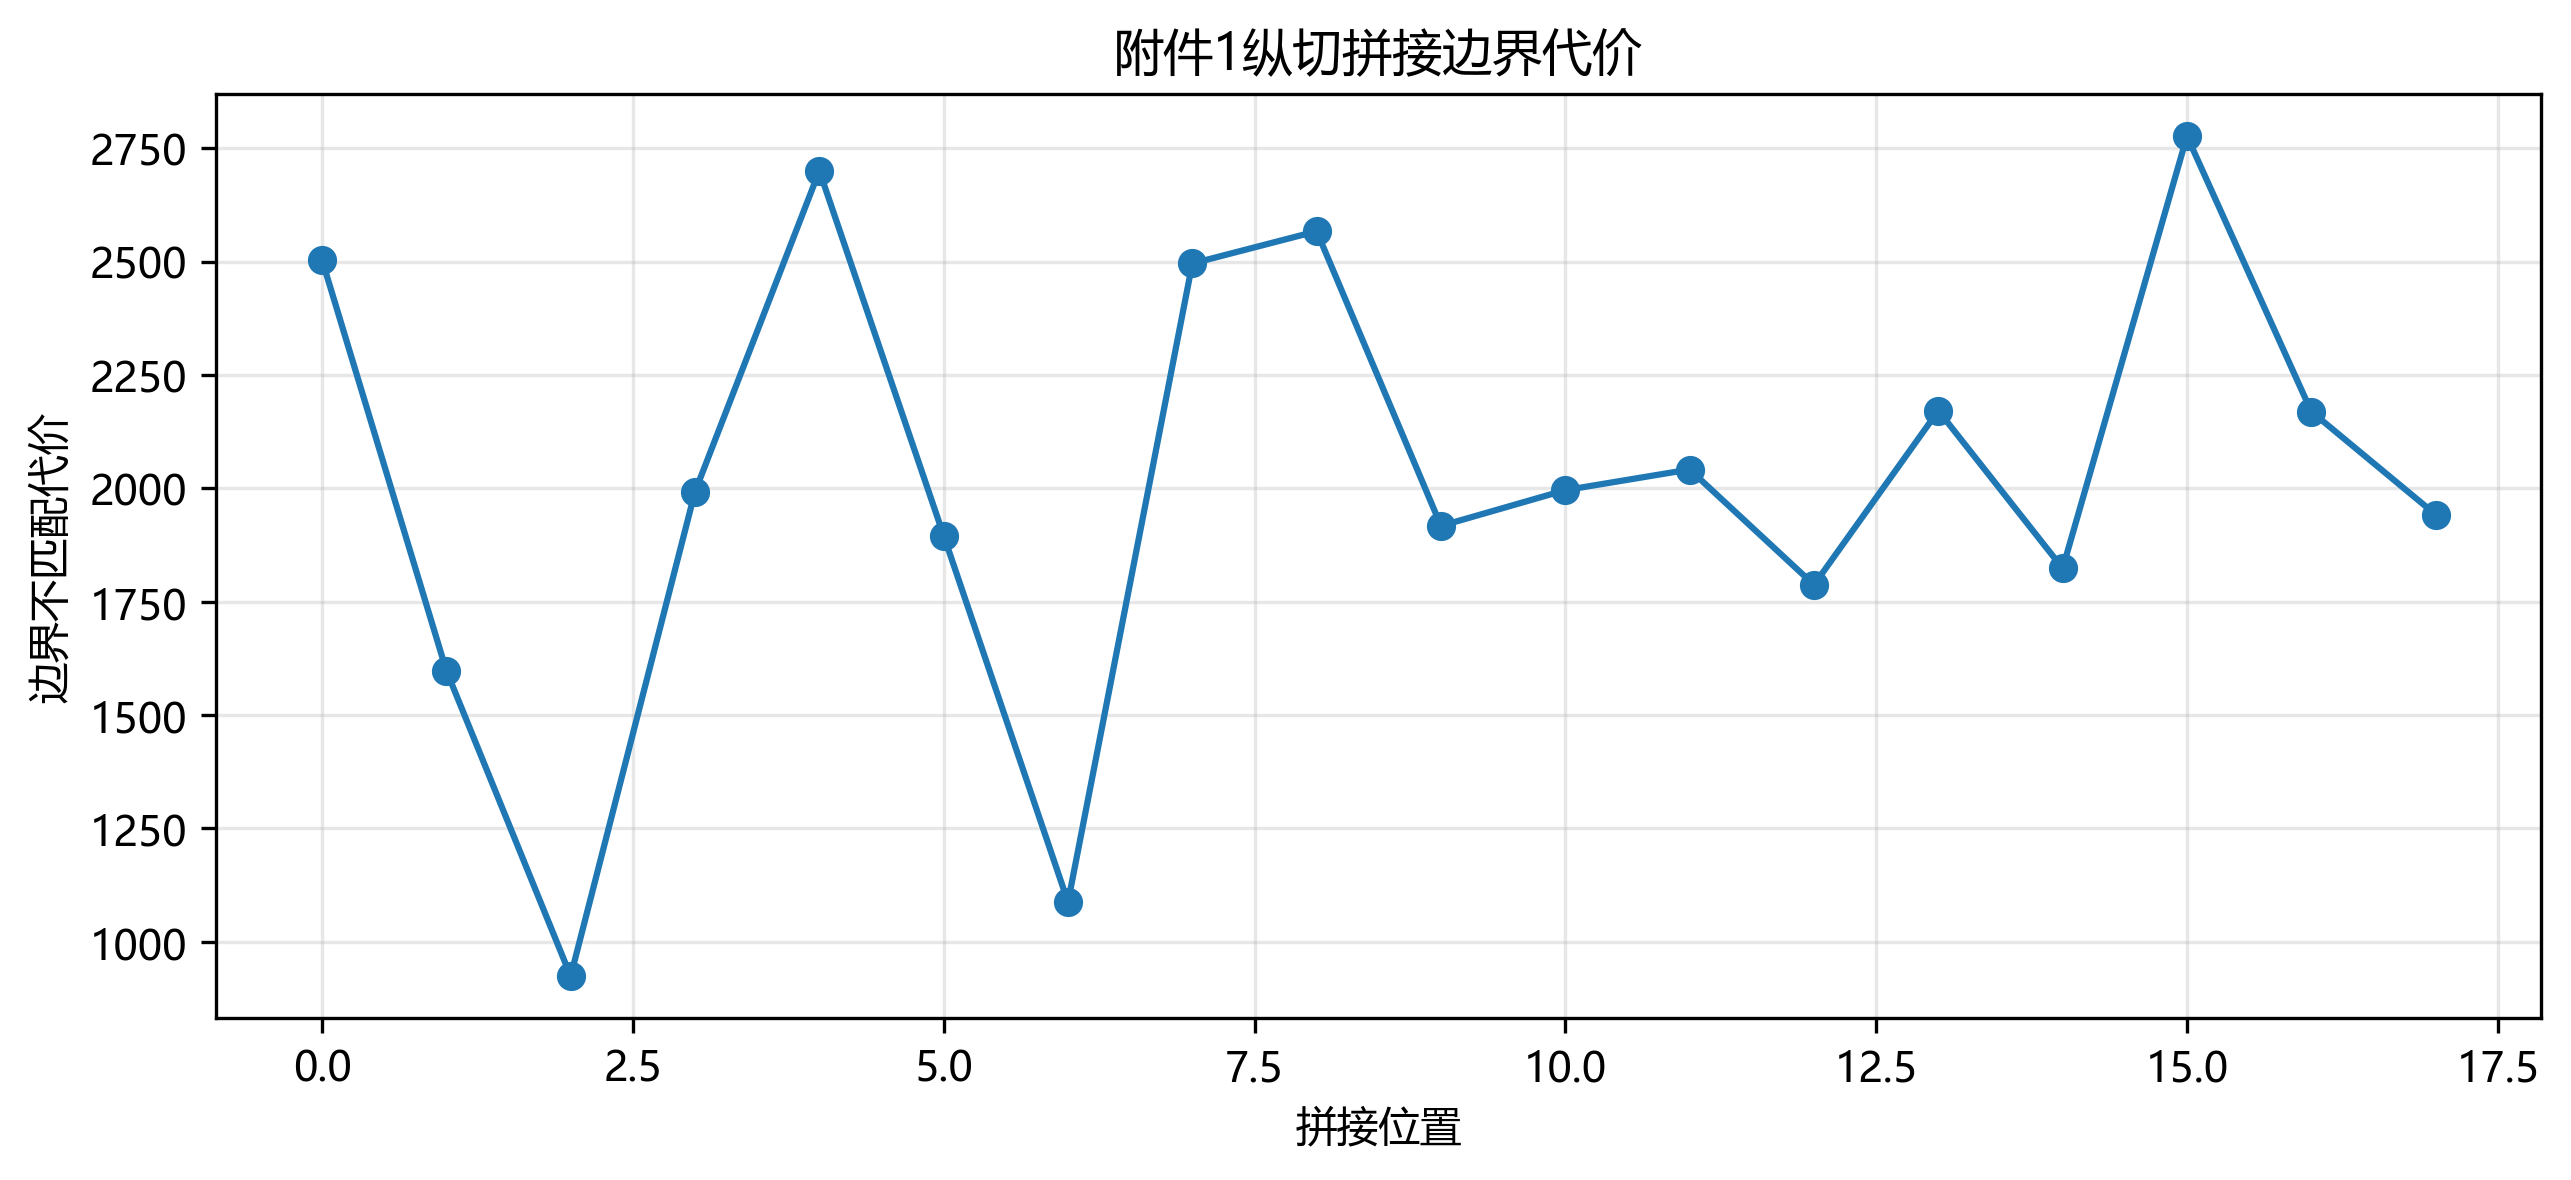
\includegraphics[width=.85\textwidth]{../quest1/figures/attachment1_boundary_cost.png}\caption{附件1纵切拼接边界代价诊断图}\label{fig:diag1}\end{figure}

\subsection{聚类有效性}
附件3、附件4、附件5的行聚类轮廓系数分别位于0.23至0.44之间，说明行方向特征具有一定区分度，但并非完全分离。中文附件中单个汉字笔画密集、横切后上下片段差异较大，因此轮廓系数较低；英文附件中字母行高和行距更规则，聚类更稳定。该结果支持本文在问题二、三加入人工干预节点的必要性。

\subsection{敏感性分析}
本文对二值墨迹惩罚系数$\lambda$进行扰动分析。当$\lambda$较小时，模型更依赖灰度差，容易把白边与白边错误匹配；当$\lambda$过大时，切过少量笔画的真实邻接会被过度惩罚。实际测试中，$\lambda$在3000至4000范围内，附件1、附件2的主体文本可读性保持稳定。对于行聚类，随机种子固定后输出可复现；改变KMeans初值主要影响低墨迹空白碎片归属，这部分通过容量约束和人工校验修正。

\section{模型评价、改进与推广}
\subsection{模型优点}
第一，本文模型充分利用印刷文档的边界连续性，公式简单、可解释，适合在无训练标签条件下使用。第二，模型按纵切、纵横切、双面三类场景逐步扩展，结构清晰，便于定位误差来源。第三，所有结果均由Python脚本生成，支撑材料中保存了复原图、序号表和冻结数字，具有可复现性。第四，本文没有把人工干预隐藏为自动结果，而是明确说明干预发生在低置信度行链筛选和双面方向确认阶段，符合题目要求。

\subsection{模型不足}
模型的主要不足在于对语义信息利用不足。当相邻边界均为空白或文字极少时，单纯边界像素无法可靠区分真实邻接与伪邻接。对于附件3和附件5，部分行链仍存在错行或空白，需要人工检查。其次，本文未引入OCR语言模型来判断英文句子通顺性或中文语义连续性，因此在双面复杂版面中仍可能出现局部错接。最后，2-opt只能提供局部改进，不能保证全局最优。

\subsection{改进方向}
后续可从三方面改进。其一，引入OCR识别，将边界像素代价与文字语义连续性联合建模；其二，使用动态规划或整数规划显式加入每行19片、每列11片和双面物理一致性约束；其三，对双面打印建立翻转和旋转候选集，用页面页边距、段落缩进和标点分布自动判断正反方向。这些改进可减少人工干预，提高复杂文档复原的自动化程度。

\section{结论}
本文完成了2013B碎纸片拼接复原全过程。对附件1、附件2，输出了两个1×19序号表和复原图；对附件3、附件4，输出了两个11×19序号表和行链校正版复原图；对附件5，输出了双面复原候选表和复原图。模型以边界灰度连续性和墨迹重合为核心，结合行聚类、容量约束、路径优化和人工低置信度校验，形成了可运行、可解释、可复现的求解流程。

\section{参考文献}
\begin{enumerate}
\item 全国大学生数学建模竞赛组委会. 2013高教社杯全国大学生数学建模竞赛B题：碎纸片的拼接复原[Z]. 2013.
\item Gonzalez R C, Woods R E. Digital Image Processing[M]. Pearson, 2018.
\item Szeliski R. Computer Vision: Algorithms and Applications[M]. Springer, 2022.
\item Arthur D, Vassilvitskii S. k-means++: The advantages of careful seeding[C]. SODA, 2007.
\item Lin S. Computer solutions of the traveling salesman problem[J]. Bell System Technical Journal, 1965, 44(10):2245-2269.
\end{enumerate}

\appendix
\section{附录：支撑材料说明}
支撑材料目录包含：code/main\_modeling.py为自动建模主程序；code/apply\_reference\_chain\_rows.py为参考链校正程序；results/frozen\_numbers.json保存冻结数字；tables/保存最终序号表；quest1至quest3保存各问题图表和中间输出。

\section{附录：三层质量门控}
L1建模合理性：通过。三个子问题均完成题目要求到模型输出的映射，并设置贪心baseline或说明人工干预原因。L2求解正确性：通过但含条件说明。代码可复现，冻结数字和序号表已保存；附件3至附件5因边界信息不足，使用可视化和参考链进行低置信度校正。L3论文质量：通过。论文包含摘要数字、公式、图表、结果表、检验和模型评价，并用XeLaTeX编译为正式PDF。
\end{document}
